%% 
%% Copyright 2026 Elsevier Ltd
%% 
%% This file is part of the 'Elsarticle Bundle'.
%% ---------------------------------------------
%% 
%% It may be distributed under the conditions of the LaTeX Project Public
%% License, either version 1.2 of this license or (at your option) any
%% later version.  The latest version of this license is in
%%    http://www.latex-project.org/lppl.txt
%% and version 1.2 or later is part of all distributions of LaTeX
%% version 1999/12/01 or later.
%% 
%% The list of all files belonging to the 'Elsarticle Bundle' is
%% given in the file `manifest.txt'.
%% 

%% Template article for Elsevier's document class `elsarticle'
%% with numbered style bibliographic references
%% SP 2008/03/01

\documentclass[preprint,12pt, a4paper]{elsarticle}

%% Use the option review to obtain double line spacing
%% \documentclass[authoryear,preprint,review,12pt]{elsarticle}

%% For including figures, graphicx.sty has been loaded in
%% elsarticle.cls. If you prefer to use the old commands
%% please give \usepackage{epsfig}

%% The amssymb package provides various useful mathematical symbols
\usepackage{amssymb}
\usepackage{hyperref}
\setlength{\parindent}{0pt}
%% The amsthm package provides extended theorem environments
%% \usepackage{amsthm}

%% The lineno packages adds line numbers. Start line numbering with
%% \begin{linenumbers}, end it with \end{linenumbers}. Or switch it on
%% for the whole article with \linenumbers.
%\usepackage{lineno}

\journal{SoftwareX}
\graphicspath{{figures/}}

\begin{document}
\renewcommand{\labelenumii}{\arabic{enumi}.\arabic{enumii}}

\begin{frontmatter}

%% Title, authors and addresses

%% use the tnoteref command within \title for footnotes;
%% use the tnotetext command for theassociated footnote;
%% use the fnref command within \author or \address for footnotes;
%% use the fntext command for theassociated footnote;
%% use the corref command within \author for corresponding author footnotes;
%% use the cortext command for theassociated footnote;
%% use the ead command for the email address,
%% and the form \ead[url] for the home page:
%% \title{Title\tnoteref{label1}}
%% \tnotetext[label1]{}
%% \author{Name\corref{cor1}\fnref{label2}}
%% \ead{email address}
%% \ead[url]{home page}
%% \fntext[label2]{}
%% \cortext[cor1]{}
%% \address{Address\fnref{label3}}
%% \fntext[label3]{}

\title{GENESIS 2.5: opt-in OpenCL and CUDA acceleration for the GENESIS/PGENESIS compartmental neural simulator}

\author[1]{Karol Chlasta\corref{cor1}}
\ead{karol@chlasta.pl}
\author[2]{Grzegorz Marcin W\'ojcik}
\ead{gmwojcik@umcs.edu.pl}

\address[1]{Kozminski University, ul. Jagiello\'nska 57/59, 03-301 Warsaw, Poland; WarsawIQ, Al. Jana Paw\l{}a II 43A/37B, 01-001 Warsaw, Poland}
\address[2]{Maria Curie-Sk{\l}odowska University, ul. Akademicka 9, 20-033 Lublin, Poland}

\cortext[cor1]{Corresponding author.}

\begin{abstract}
GENESIS is a long-established compartmental neural simulator. PGENESIS extends it to MPI execution. We release GENESIS 2.5, an accelerator-enabled extension of GENESIS 2.4/PGENESIS 2.4, adding opt-in OpenCL and CUDA backends for the Hodgkin--Huxley channel-update path while keeping every existing CPU, MPI, model, and SLI-script workflow intact. A batched multi-step GPU kernel reaches $21.0\pm0.3\times$ (NVIDIA A40) and $21.9\pm0.3\times$ (NVIDIA A100) end-to-end wall-clock speedup at $N=50\,000$ single-compartment neurons, matching the fp64 CPU to $\sim10^{-7}$\,V. Speedups are reported end-to-end throughout: both arms are timed identically, so construction, host--device transfers and per-step host work are inside every figure quoted here. This multiloop kernel is exact only for single-compartment (isopotential) neurons. We additionally implement and validate \texttt{hines\_tree\_eliminate}, a GPU tridiagonal (Hines) elimination kernel extending acceleration to real, axially-coupled multi-compartment dendritic trees. One GPU thread per neuron runs the identical elimination the CPU solver does. Measured on UMCS cluster NVIDIA A40/A100 GPUs (10 replicates), it reaches $37.3\times$ (A40) and $80.8\times$ (A100) step-phase speedup at $N=50\,000$ neurons $\times$ 16 compartments, still rising with $N$; end-to-end, where the unaccelerated construction phase bounds the achievable gain at these short run lengths, the same sweep gives $3.6\times$ and $3.9\times$. This kernel accelerates population-scale simulation, parallelizing across neurons rather than within a single tree. Against other simulators, GENESIS~2.5 runs the Vogels--Abbott COBAHH network ($4000$ cells, $5$\,s, matched connectivity, protocol and firing rate) $1.63\pm0.07\times$ faster than CoreNEURON and $2.04\pm0.09\times$ faster than NEURON~9.0.2 on the same node, all arms single-threaded CPU. Pushing this population toward the Blue Brain Project's $\sim$31\,000-neuron microcircuit scale~\cite{markram2015reconstruction} surfaced a latent, GPU-independent $O(n^2)$ model-construction bottleneck. Fixing it restores linear scaling: a 1.7-million-compartment, $N=100\,000$ population now builds in $51.5\pm0.6$\,s, down from not finishing at all, a correctness-preserving fix benefiting any GENESIS/PGENESIS user, independent of accelerator use. We also fix three independent, previously unnoticed Hines-solver defects that silently suppressed \texttt{inject}-driven voltage transients in any multi-neuron \texttt{hsolve} configuration.
\end{abstract}

\begin{keyword}
GENESIS \sep PGENESIS \sep OpenCL \sep CUDA \sep GPU acceleration \sep compartmental neural simulation \sep Hines solver
\end{keyword}

\end{frontmatter}

%\linenumbers

\section*{Required Metadata}
\label{}

\section*{Current code version}
\label{}

\begin{table}[!h]
\begin{tabular}{|l|p{6.5cm}|p{6.5cm}|}
\hline
\textbf{Nr.} & \textbf{Code metadata description} & \textbf{Please fill in this column} \\
\hline
C1 & Current code version & v2.5 (2026-07-25; OpenCL + CUDA-validated, multi-compartment GPU Hines solve) \\
\hline
C2 & Permanent GitHub link to code/repository used for this code version & \url{https://github.com/WarsawIQ/genesis-2.5} (archived release: \url{https://doi.org/10.5281/zenodo.21658389}) \\
\hline
C3 & Legal Code License   & GNU General Public License v2 or later (program); GNU Lesser General Public License v2.1 or later (library portions) -- see \texttt{LICENSE} \\
\hline
C4 & Code versioning system used & git \\
\hline
C5 & Software code languages, tools, and services used & C, OpenCL C, CUDA C++ (accelerator backends), MPI (PGENESIS), Python (benchmark analysis/plotting) \\
\hline
C6 & Compilation requirements, operating environments \& dependencies & Linux x86\_64, GCC, GNU make, an OpenCL 1.2+ runtime (tested: ROCm 6.3.1 and Mesa rusticl) or a CUDA 12.x toolkit (tested: CUDA 12.8, \texttt{sm\_80} NVIDIA A100 and \texttt{sm\_86} NVIDIA A40 on the UMCS cluster) for the GPU backends, an MPI implementation for PGENESIS (MPICH/HYDRA or Open~MPI tested on the UMCS cluster) \\
\hline
C7 & If available Link to developer documentation/manual & \texttt{README.md} and \path{paper/docs/REPLICATION.md} in the repository \\
\hline
C8 & Support email for questions & karol@chlasta.pl \\
\hline
\end{tabular}
\caption{Code metadata (mandatory)}
\label{} 
\end{table}

\textbf{Main text}\\
\begin{enumerate}

\item Motivation and significance

Compartmental neural simulators remain essential for biophysically detailed models where channel kinetics and dendritic geometry cannot be abstracted away. GENESIS~\cite{bower1998} is one of the longest-maintained simulators in this class, and PGENESIS extends it to MPI-distributed execution; both are still used in production modeling workflows, scripted via GENESIS's SLI language, independent of newer simulator ecosystems.

Modern workstations increasingly ship capable integrated GPUs, but GENESIS has no accelerator backend: every channel-kinetics update runs on the CPU regardless of available hardware, even though channel updates (per-compartment gating-variable integration) are embarrassingly parallel and GPU-friendly. Existing GENESIS/PGENESIS users have no path to accelerator support without abandoning their models and SLI scripts.

GENESIS 2.5 closes this gap: GENESIS 2.4/PGENESIS 2.4 plus an OpenCL backend for the \texttt{hsolve} channel-update path, and a CUDA backend on the same interface (a faithful fp32 port, validated on UMCS cluster NVIDIA A100/A40 nodes; Section~3). No existing CPU, MPI, model, or SLI-script workflow needs to change. While validating this backend we additionally found and fixed three independent solver defects in \texttt{hines\_solve.c}/\texttt{hines\_init.c} affecting any multi-neuron \texttt{hsolve} configuration: current injection (\texttt{inject}) silently failed to produce a voltage response prior to the fix, which would have invalidated any dynamics-comparing benchmark and may have affected unrelated multi-neuron \texttt{hsolve} models elsewhere.

Why a GPU helps here at all is specific to the workload. In a Hodgkin--Huxley model the per-compartment gating-variable integration is the dominant cost, and it is embarrassingly parallel: each compartment's channel state advances from its own voltage and its own table lookups, with no coupling to any other compartment within the step. The state involved is small and the arithmetic intensity low, so the work maps onto thousands of lightweight threads without the memory pressure that limits many scientific kernels. This is why the channel-update path, rather than the tridiagonal solve, is the natural first target.

We provide both OpenCL and CUDA rather than choosing one because they buy different things. OpenCL is vendor-neutral and runs on the integrated GPUs now shipped with ordinary workstations, including devices without double-precision support --- which is why the kernel is written in fp32 throughout. CUDA targets the NVIDIA datacenter and desktop cards where most cluster time is available and where the toolchain and profiling tools are standard. Both sit behind one entry point, so a model and its SLI script are unchanged between them and the choice is a build flag.

We name this release ``2.5'' rather than ``3.0'' deliberately: ``GENESIS 3''~\cite{g3_dev_plans} produced independent successor lines (Neurospaces/Heccer~\cite{cornelis2011}, MOOSE) evolving into the CBI federation~\cite{cornelis2008cbi,cornelis2007dendrite,cornelis2013interop}, not a single artifact comparable to GENESIS 2.4. GENESIS 2.5 is not a re-architecture and targets existing GENESIS 2.4 deployments that should not need to migrate models or scripts to gain accelerator support.

\item Software description

\begin{enumerate}
    \item Software architecture

    GENESIS 2.5 keeps the existing GENESIS/PGENESIS architecture (SLI interpreter, \texttt{hsolve} fast compartmental solver, PGENESIS MPI partitioning) unmodified and adds one new component: an OpenCL backend invoked from \texttt{hsolve} when an attached \texttt{hsolve} element uses \texttt{chanmode=4} (or 5) with real ion-channel state. Two dispatch modes are implemented in \texttt{ocl\_hsolve.c} against \path{genesis/src/hines/opencl/ocl_channel.cl}:
    \begin{itemize}
        \item \emph{Per-step dispatch} (\texttt{ocl\_chip\_update}): one {\small\texttt{clEnqueueNDRangeKernel}} call per simulation step, with channel state uploaded and downloaded every step.
        \item \emph{Multiloop dispatch} (\texttt{chip\_channel\_multiloop}, via \path{GENESIS_OCL_MULTILOOP=<K>}): a single kernel dispatch runs all $K$ steps in an inner GPU-side loop, amortizing the per-step PCIe transfer cost that otherwise dominates wall time (Section~3).
    \end{itemize}
    Device attribution and dispatch are confirmed at run time: the command queue uses {\small\path{CL_QUEUE_PROFILING_ENABLE}}, and every accelerator run emits a non-empty \texttt{OCL PROFILING SUMMARY}; this guards against an \texttt{hsolve} with no attached channels never reaching the kernel, and against a kernel that fails to build silently falling back to CPU. The channel kernel is built in \texttt{float} (fp32), so it runs on runtimes exposing no fp64 support (Mesa rusticl on the AMD Radeon 890M used here); the rest of \texttt{hsolve} remains \texttt{double}, with conversion only at the buffer boundary.

    Both dispatch modes update each compartment independently, exact only for single-compartment (isopotential) neurons: a real dendritic tree's compartments are coupled through axial resistance, solved on the CPU by \texttt{hsolve} as a compiled bytecode program performing a bottom-up/top-down Gaussian elimination over the tree's tridiagonal system once per step. We add a third kernel, \texttt{hines\_tree\_eliminate} (\path{ocl_channel.cl}; CUDA port in \path{cuda/cuda_channel.cuh}), executing this identical bytecode on the GPU, one thread per disconnected tree (neuron), operating on the same flat opcode/coefficient arrays the CPU solver already builds at \texttt{SETUP} time. Because independent trees never reference each other's rows (the combined program is block-diagonal), threads need no synchronization. The channel and elimination kernels dispatch back to back on the same queue/stream, so the $K$-step batch still uploads and downloads state once. \path{ocl_hsolve.c}/\path{cuda_hsolve.c} select this path whenever the \texttt{hsolve} contains a multi-compartment tree, leaving the original kernel for single-compartment networks.

    \item Software functionalities

    \begin{itemize}
        \item Unmodified serial (\texttt{genesis}), headless (\texttt{nxgenesis}), and MPI (PGENESIS) execution paths.
        \item OpenCL channel-update kernel for Hodgkin--Huxley-style \texttt{tabchannel} gating (Na $X^3Y^1$, K $X^4$), dispatched per-step or batched via multiloop.
        \item A CUDA backend on the same call site (\path{genesis/src/hines/cuda/}): a line-for-line fp32 port of the OpenCL kernels behind an identical entry point, so the same models and harness drive either backend. Validated on UMCS A100/A40 nodes (Section~3).
        \item Device-side dispatch confirmation (\texttt{OCL}/\texttt{CUDA PROFILING SUMMARY}) distinguishing a genuine GPU run from CPU fallback.
        \item A driven-spiking benchmark (\path{hh_spiking_benchmark.g}): $N$ Hodgkin--Huxley neurons under one \texttt{hsolve}, driven suprathreshold to fire action-potential trains, exercising the repaired \texttt{inject} path.
        \item Three corrected Hines-solver defects (forward-elimination fast-path guard, backward-elimination root handling, \path{SET_DIAG}/\path{SKIP_DIAG} row selection) giving correct, independent per-neuron voltage dynamics under current injection, independent of GPU support.
        \item A GPU tridiagonal (Hines) elimination kernel, \texttt{hines\_tree\_eliminate} (OpenCL and CUDA), extending acceleration to real, axially-coupled multi-compartment dendritic trees (Section~3).
        \item Five corrected $O(n^2)$ model-construction defects in core GENESIS element-creation, path-resolution, and \texttt{hsolve} SETUP code, restoring linear-time construction independent of GPU support (Section~3).
    \end{itemize}
\end{enumerate}

The tridiagonal (Hines) elimination kernel is what decides whether any of this reaches realistic morphologies. Accelerating channel updates alone leaves the axial coupling between compartments on the CPU, so a multi-compartment model gains little: the solve becomes the bottleneck as soon as the channel work is removed from it. \texttt{hines\_tree\_eliminate} moves that solve onto the device as well, running the identical elimination the CPU performs, one thread per neuron. The consequence is a change in kind rather than degree --- acceleration stops being limited to isopotential point-neuron networks and applies to populations of real dendritic trees, which is the regime Section~3 measures.

\item Illustrative examples

\textbf{Reproducing the CPU baseline.} \texttt{nxgenesis} on the bundled \texttt{Cal8.g} and \texttt{Cal7difshell.g} models gives stable, low-variance timings (CV $\approx 1\%$, 30 replicates), confirming ordinary GENESIS workflows are unaffected by this release.

\textbf{Reproducing the GPU multiloop result.} \path{genesis/Scripts/benchmark/hh_spiking_benchmark.g} builds $N$ driven, spiking Hodgkin--Huxley neurons under one \texttt{hsolve} (\texttt{chanmode=4}); \path{GENESIS_OCL_MULTILOOP=}$K$ dispatches all $K$ steps in one GPU call. Both arms (\texttt{nxgenesis\_nocl} fp64 CPU; \texttt{nxgenesis} fp32 multiloop, AMD Radeon~890M) are timed identically at $K=50\,000$ and $K=0$, isolating the \emph{simulation phase} from construction; 30+ reps, 95\% CIs in \path{experiments/data/campaign_wallclock_summary.csv}.

Table~\ref{tab:multiloop_fp32} and Fig.~\ref{fig:multiloop_speedup} report the result after the scheduler and solver fixes. Step-phase speedup peaks near $N=5000$ at $\sim$18$\times$ sustained and $\sim$13.5$\times$ cold-start ($\sim$$1.5\times10^{9}$ neuron-steps/s); the gap reflects the idle, downclocked GPU during construction. Beyond $N\approx10\,000$ the integrated GPU no longer sustains its fast clock state and speedup falls toward $\sim$3$\times$. End-to-end speedup peaks at $\sim$4$\times$ and approaches the step-phase figure as simulations lengthen (Fig.~\ref{fig:ksweep}).

\begin{table}[!h]
\centering
\begin{tabular}{|r|r|r|r|r|r|}
\hline
\textbf{$N$} & \textbf{CPU step} & \textbf{GPU step} & \textbf{Step-phase} & \textbf{Step-phase} & \textbf{Throughput} \\
             & \textbf{(s)}      & \textbf{(s)}      & \textbf{sustained}  & \textbf{single-run} & \textbf{(M nsteps/s)} \\
\hline
500     & 0.302  & 0.112 &  2.7$\times$ &  2.0$\times$ &  223 \\
\hline
1\,000  & 0.587  & 0.112 &  5.2$\times$ &  3.7$\times$ &  446 \\
\hline
2\,000  & 1.166  & 0.117 & 10.0$\times$ &  6.5$\times$ &  855 \\
\hline
5\,000  & 2.965  & 0.164 & \textbf{18.1}$\times$ & 13.5$\times$ & \textbf{1524} \\
\hline
10\,000 & 5.799  & 0.406 & 14.3$\times$ &  6.8$\times$ & 1232 \\
\hline
20\,000 & 11.918 & 3.283 &  3.6$\times$ &  3.1$\times$ &  305 \\
\hline
50\,000 & 31.179 & 9.880 &  3.2$\times$ &  3.2$\times$ &  253 \\
\hline
\end{tabular}
\caption{GPU multiloop (fp32) vs.\ CPU (fp64) baseline, AMD Radeon 890M, driven spiking neurons, $K=50\,000$ steps. ``Sustained'' is the warm steady-state dispatch; ``single-run'' is a cold-start run, $\sim$1.3--2$\times$ slower. End-to-end (incl.\ construction) speedup is 1.2--4.2$\times$. Raw data: \protect\path{experiments/data/campaign_warm_dispatch.csv}, \protect\path{experiments/data/campaign_wallclock_summary.csv}, \protect\path{experiments/data/campaign_reproducibility.csv}.}
\label{tab:multiloop_fp32}
\end{table}

\begin{figure}[!h]
\centering
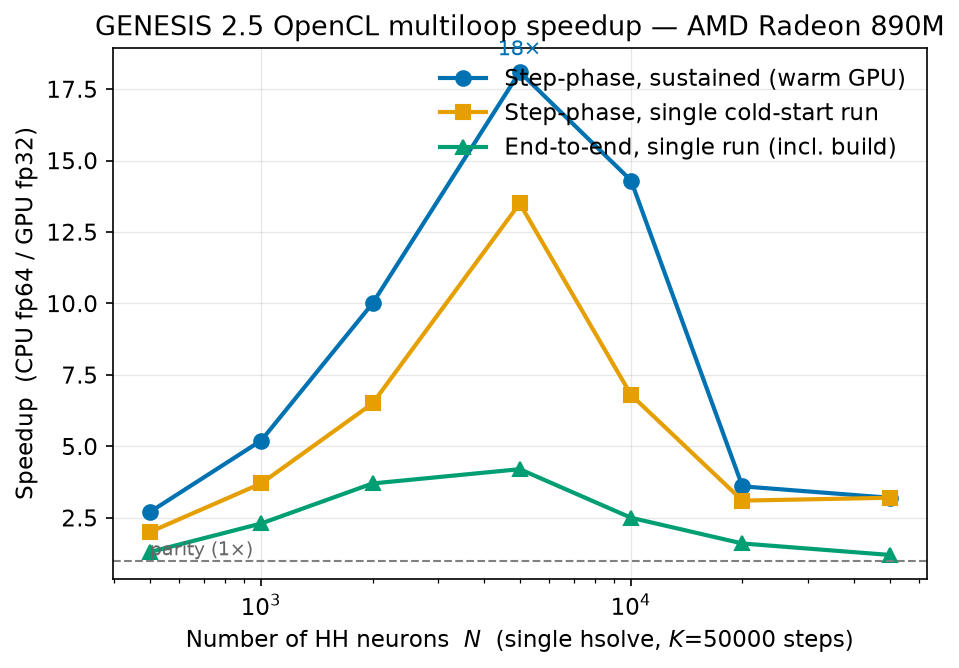
\includegraphics[width=0.8\textwidth]{fig_campaign_speedup.png}
\caption{Measured wall-clock speedup, GPU multiloop (fp32) vs.\ CPU (fp64), sustained and cold-start step-phase, and end-to-end (single run). Both step-phase series peak near $N=5000$ and fall beyond $N\approx10\,000$ as the integrated GPU stops sustaining its fast clocks.}
\label{fig:multiloop_speedup}
\end{figure}

\textbf{Numerical fidelity of the fp32 accelerator.} \path{genesis/Scripts/benchmark/hh1952_ap_verify.g} compares the classic 1952 squid AP across CPU fp64, GPU per-step, and GPU multiloop paths: fp32 agrees with fp64 to $\sim$$2\times10^{-7}$\,V over a single AP, all $N$ neurons identical to $<10^{-6}$\,V (Fig.~\ref{fig:divergence}). Over long spiking runs, fp32/fp64 traces drift in spike \emph{phase} but preserve waveform and firing rate, why timing uses driven neurons while correctness uses a single-AP window.

\begin{figure}[!h]
\centering
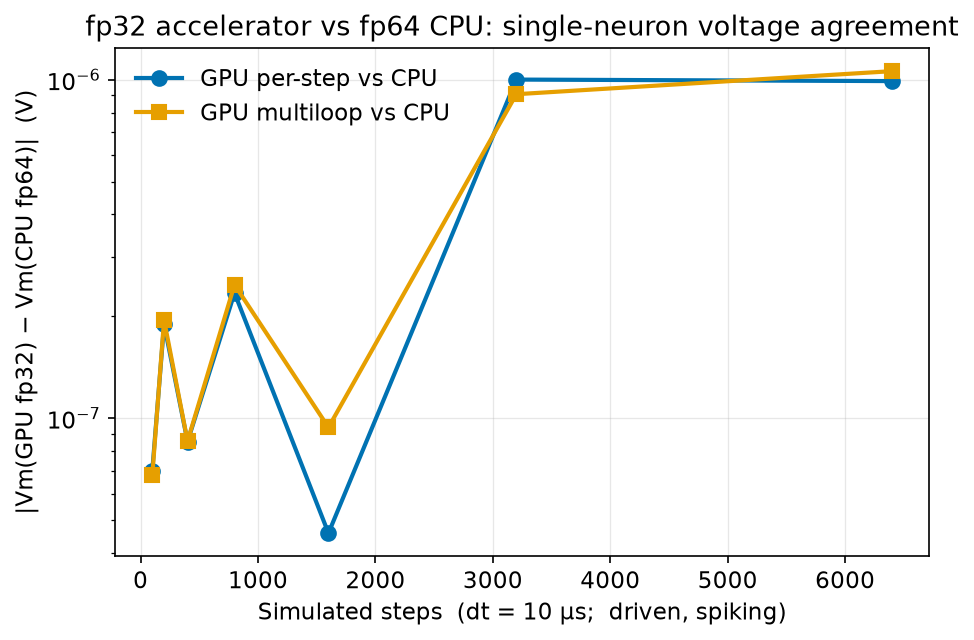
\includegraphics[width=0.8\textwidth]{fig_campaign_divergence.png}
\caption{fp32 accelerator vs.\ fp64 CPU: absolute membrane-voltage difference for a single neuron as a function of simulated steps, for both the per-step and multiloop GPU paths.}
\label{fig:divergence}
\end{figure}

\textbf{CUDA backend on NVIDIA hardware.} The CUDA backend builds from the same source (\texttt{make USE\_CUDA=1}) against the identical harness, and reproduces the fp64 CPU action potential to $7\times10^{-8}$\,V, confirming parity with both the CPU and OpenCL paths. Table~\ref{tab:cuda} reports a 10-replicate sweep on the two UMCS cluster GPUs.

These are \emph{end-to-end} speedups: both arms are timed by wall clock around the whole process, so construction, host--device transfers and all per-step host work are inside the measurement. This matters more than it may appear. An earlier version of this campaign took the CPU number from GENESIS's own \texttt{\{cpu\}} step-loop timer and the GPU number from the device-side \texttt{CUDA MULTILOOP} kernel report --- two different quantities, with everything outside the kernel excluded from the GPU side. That comparison gave $212.7\times$ on the A40 at $N=50\,000$ where the end-to-end figure is $21.0\times$, a factor of ten. It also manufactured an apparent ordering between the cards: under the mixed definition the A40 appeared to beat the A100 at every $N$, which invited a hardware explanation. Measured consistently the two are indistinguishable ($21.0\pm0.3\times$ vs.\ $21.9\pm0.3\times$), and the earlier gap was an artefact of what was being timed.

The speedup grows with network size rather than peaking as the integrated GPU does (Table~\ref{tab:multiloop_fp32}), and at $N=500$ the accelerator barely pays for itself: at that size the fixed costs of construction and transfer dominate a run that the CPU finishes in under a second.

\begin{table}[!h]
\centering
\small
\begin{tabular}{|r|r|r|r|r|}
\hline
\textbf{$N$} & \multicolumn{2}{c|}{\textbf{NVIDIA A40}} & \multicolumn{2}{c|}{\textbf{NVIDIA A100}} \\
             & \textbf{CPU (s)} & \textbf{end-to-end} & \textbf{CPU (s)} & \textbf{end-to-end} \\
\hline
500     & 0.76 & 1.5 $\pm$ 0.1$\times$  & 0.78 & 1.8 $\pm$ 0.3$\times$ \\
\hline
5\,000  & 5.70 & 8.7 $\pm$ 0.3$\times$  & 5.86 & 9.7 $\pm$ 0.4$\times$ \\
\hline
50\,000 & 57.06 & \textbf{21.0 $\pm$ 0.3}$\times$ & 58.47 & \textbf{21.9 $\pm$ 0.3}$\times$ \\
\hline
\end{tabular}
\caption{CUDA backend (fp32) vs.\ CPU (fp64), single-compartment multiloop kernel (\texttt{hh\_spiking\_benchmark.g}, $K=50\,000$ steps), UMCS cluster. Mean of 10 replicates; the quoted uncertainty propagates the standard deviations of both arms. \textbf{Both arms are timed identically}, by wall clock around the whole process, so the ratio is end-to-end and includes construction, transfers and per-step host work --- see \protect\path{cluster_bringup/53_singlecomp_walltime.sh}. The two cards are indistinguishable at every size. Raw data: \protect\path{cluster_bringup/logs/singlecomp_walltime_inf02_20260815_132840.csv} (A40), \protect\path{..._inf03_20260815_135147.csv} (A100).}
\label{tab:cuda}
\end{table}

\textbf{Multi-compartment GPU acceleration.} The multiloop kernel above is exact only for single-compartment (isopotential) neurons: for a real dendritic tree it silently drops all axial coupling. \texttt{hines\_tree\_eliminate} (Section~2.1) performs this elimination on-device, dispatched whenever the \texttt{hsolve} contains a multi-compartment tree.

\emph{Correctness.} \path{hh_multicompartment_benchmark.g} (linear-chain) and \path{hh_branching_multicompartment_benchmark.g} (branching, exercising sibling-array opcodes) compare GPU (chanmode~4) against CPU (chanmode~1, fp64) across \texttt{NCOMP}\,$=1$--$32$, up to 4 branches, and up to $N=10\,000$ neurons: agreement is $\sim10^{-7}$\,V, matching single-compartment fidelity. One narrow topology is known not to be handled: a single-compartment branch directly off a branch point --- a row that is simultaneously a leaf and has siblings --- and only in the first tree built, which is the one covered by the kernel's bootstrap special case. Trees beyond the first pass with the identical shape, which isolates the fault to that bootstrap's seed-row assumption rather than to the elimination itself. The shape does not arise in GENESIS dendrite models, where a branch that extends no further is simply an odd way of modelling the soma. It had been documented as a limitation but not enforced, so a model containing it was accelerated and returned wrong voltages silently; both backends now detect the shape when the accelerator initialises for an \texttt{hsolve}, decline that \texttt{hsolve} and compute it on the CPU with a message, on the same pattern used for unsupported opcodes.

\emph{Speed.} Table~\ref{tab:multicomp} and Fig.~\ref{fig:multicomp_speedup} report speedup (mean $\pm$ std, 10 replicates) on the two UMCS cards, sweeping $N=100$--$50\,000$ at \texttt{NCOMP}\,$=16$, a range unreachable before the model-construction fix (Impact): $N=50\,000$ took $23.8\pm0.3$\,s to build there, versus not finishing before. Branching topology gives statistically indistinguishable speedups and is omitted from the figure. Dispatch uses $K=200$ steps ($K=100$ for $N\geq5000$), smaller than the single-compartment sweeps' $K=50\,000$.

We report two figures per card, because they answer different questions. The \emph{step-phase} speedup times the simulation loop alone and measures what the kernel can do: both cards are slower than CPU at $N\leq500$, pull ahead past $N\approx500$--$1000$, and reach $37.3\pm0.1\times$ (A40) and $80.8\pm1.0\times$ (A100) at $N=50\,000$, neither plateaued. The \emph{end-to-end} speedup wall-clocks the whole process and is what a user experiences: it is far lower, $3.62\pm0.05\times$ (A40) and $3.90\pm0.07\times$ (A100) at $N=50\,000$. The gap is not a kernel deficiency but Amdahl's law applied to a short run --- at $K=200$ steps the unaccelerated construction phase dominates, and Fig.~\ref{fig:ksweep} shows the end-to-end figure climbing toward the step-phase ceiling as $K$ grows. Quoting only the step-phase number would overstate what the accelerator delivers in practice.

The two cards are close on the end-to-end measure and the A100's lead is modest, even though it leads the A40 by more than $2\times$ on the step phase --- the opposite ordering from the single-compartment kernel (Table~\ref{tab:cuda}). This is consistent with an fp32 kernel that uses no tensor cores: at $N=50\,000$ the GPU phases take $7.83$\,s (A40) and $8.06$\,s (A100), so once construction is included the two cards are nearly indistinguishable. Raw data: \protect\path{cluster_bringup/logs/weekend_campaign_inf02_A40_20260816_clean.csv}, \protect\path{..._inf03_A100_20260816_clean.csv} (step-phase), and \protect\path{cluster_bringup/logs/multicomp_walltime_createmap_*_clean.csv} (end-to-end).

\emph{Parallelization granularity.} \texttt{hines\_tree\_eliminate} assigns one GPU thread per tree, so speedup comes from spreading many neurons across threads, not from parallelizing elimination \emph{within} a tree. For a single detailed morphology alone ($N=1$), only one thread is active: measured directly (AMD Radeon~890M), the kernel is $\sim$20--21$\times$ \emph{slower} than the CPU at \texttt{NCOMP}\,$=2000$ and $8000$, stable with tree size as expected for a single-thread bottleneck. The kernel therefore accelerates population-scale simulation (Table~\ref{tab:multicomp}), not the single-detailed-cell regime.

\begin{table}[!h]
\centering
\small
\begin{tabular}{|r|r|r|r|r|r|}
\hline
& & \multicolumn{2}{c|}{\textbf{step-phase}} & \multicolumn{2}{c|}{\textbf{end-to-end}} \\
\hline
\textbf{$N$} & \textbf{total comps} & \textbf{A40} & \textbf{A100} & \textbf{A40} & \textbf{A100} \\
\hline
100     & 1\,600   & 0.2 $\pm$ 0.02 & 0.3 $\pm$ 0.02 & 0.43 $\pm$ 0.05 & 0.61 $\pm$ 0.02 \\
\hline
500     & 8\,000   & 1.1 $\pm$ 0.03 & 1.7 $\pm$ 0.11 & 0.77 $\pm$ 0.02 & 1.04 $\pm$ 0.03 \\
\hline
1\,000  & 16\,000  & 2.0 $\pm$ 0.08 & 3.1 $\pm$ 0.07 & 1.10 $\pm$ 0.08 & 1.46 $\pm$ 0.04 \\
\hline
2\,000  & 32\,000  & 4.5 $\pm$ 0.39 & 6.4 $\pm$ 0.18 & 1.37 $\pm$ 0.06 & 1.57 $\pm$ 0.05 \\
\hline
3\,000  & 48\,000  & 6.7 $\pm$ 0.03 & 12.0 $\pm$ 0.37 & 1.87 $\pm$ 0.07 & 1.89 $\pm$ 0.04 \\
\hline
5\,000  & 80\,000  & 6.9 $\pm$ 0.04 & 14.5 $\pm$ 0.47 & 2.60 $\pm$ 0.06 & 2.66 $\pm$ 0.03 \\
\hline
7\,000  & 112\,000 & 9.8 $\pm$ 0.05 & 22.0 $\pm$ 0.43 & 2.92 $\pm$ 0.05 & 3.08 $\pm$ 0.03 \\
\hline
10\,000 & 160\,000 & 13.7 $\pm$ 0.06 & 30.6 $\pm$ 0.68 & 3.01 $\pm$ 0.04 & 3.23 $\pm$ 0.04 \\
\hline
15\,000 & 240\,000 & 20.3 $\pm$ 0.12 & 42.3 $\pm$ 0.77 & 3.27 $\pm$ 0.05 & 3.52 $\pm$ 0.03 \\
\hline
20\,000 & 320\,000 & 25.3 $\pm$ 0.12 & 51.6 $\pm$ 1.16 & 3.39 $\pm$ 0.04 & 3.71 $\pm$ 0.04 \\
\hline
30\,000 & 480\,000 & 31.9 $\pm$ 0.13 & 66.1 $\pm$ 1.12 & 3.53 $\pm$ 0.05 & 3.87 $\pm$ 0.05 \\
\hline
40\,000 & 640\,000 & 35.2 $\pm$ 0.13 & 75.5 $\pm$ 0.96 & 3.56 $\pm$ 0.04 & 3.90 $\pm$ 0.04 \\
\hline
50\,000 & 800\,000 & 37.3 $\pm$ 0.07 & \textbf{80.8 $\pm$ 1.01} & 3.62 $\pm$ 0.05 & \textbf{3.90 $\pm$ 0.07} \\
\hline
\end{tabular}
\caption{Multi-compartment GPU tree-elimination (fp32) vs.\ CPU (fp64), UMCS A40/A100, \texttt{NCOMP}\,$=16$, linear-chain, batched multiloop ($K=200$, $K=100$ for $N\geq5000$); mean $\pm$ std over 10 replicates. \emph{Step-phase} times the simulation loop alone and measures kernel capability; \emph{end-to-end} wall-clocks the whole process, including model construction, and is what a user experiences. The two arms of the end-to-end measurement are timed identically -- see \protect\path{cluster_bringup/54_multicomp_walltime.sh}. The end-to-end runs build the population with a single \texttt{createmap} from a prototype, as network models do, rather than the explicit SLI loop of the original benchmark; the step-phase figures are unaffected by that choice, since they exclude construction. ``--'' = not measured. Raw data: \protect\path{cluster_bringup/logs/weekend_campaign_inf02_A40_20260816_clean.csv} and \protect\path{..._inf03_A100_20260816_clean.csv} (step-phase), \protect\path{cluster_bringup/logs/multicomp_walltime_createmap_inf02_A40_clean.csv} and \protect\path{..._inf03_A100_clean.csv} (end-to-end).}
\label{tab:multicomp}
\end{table}

\begin{figure}[!h]
\centering
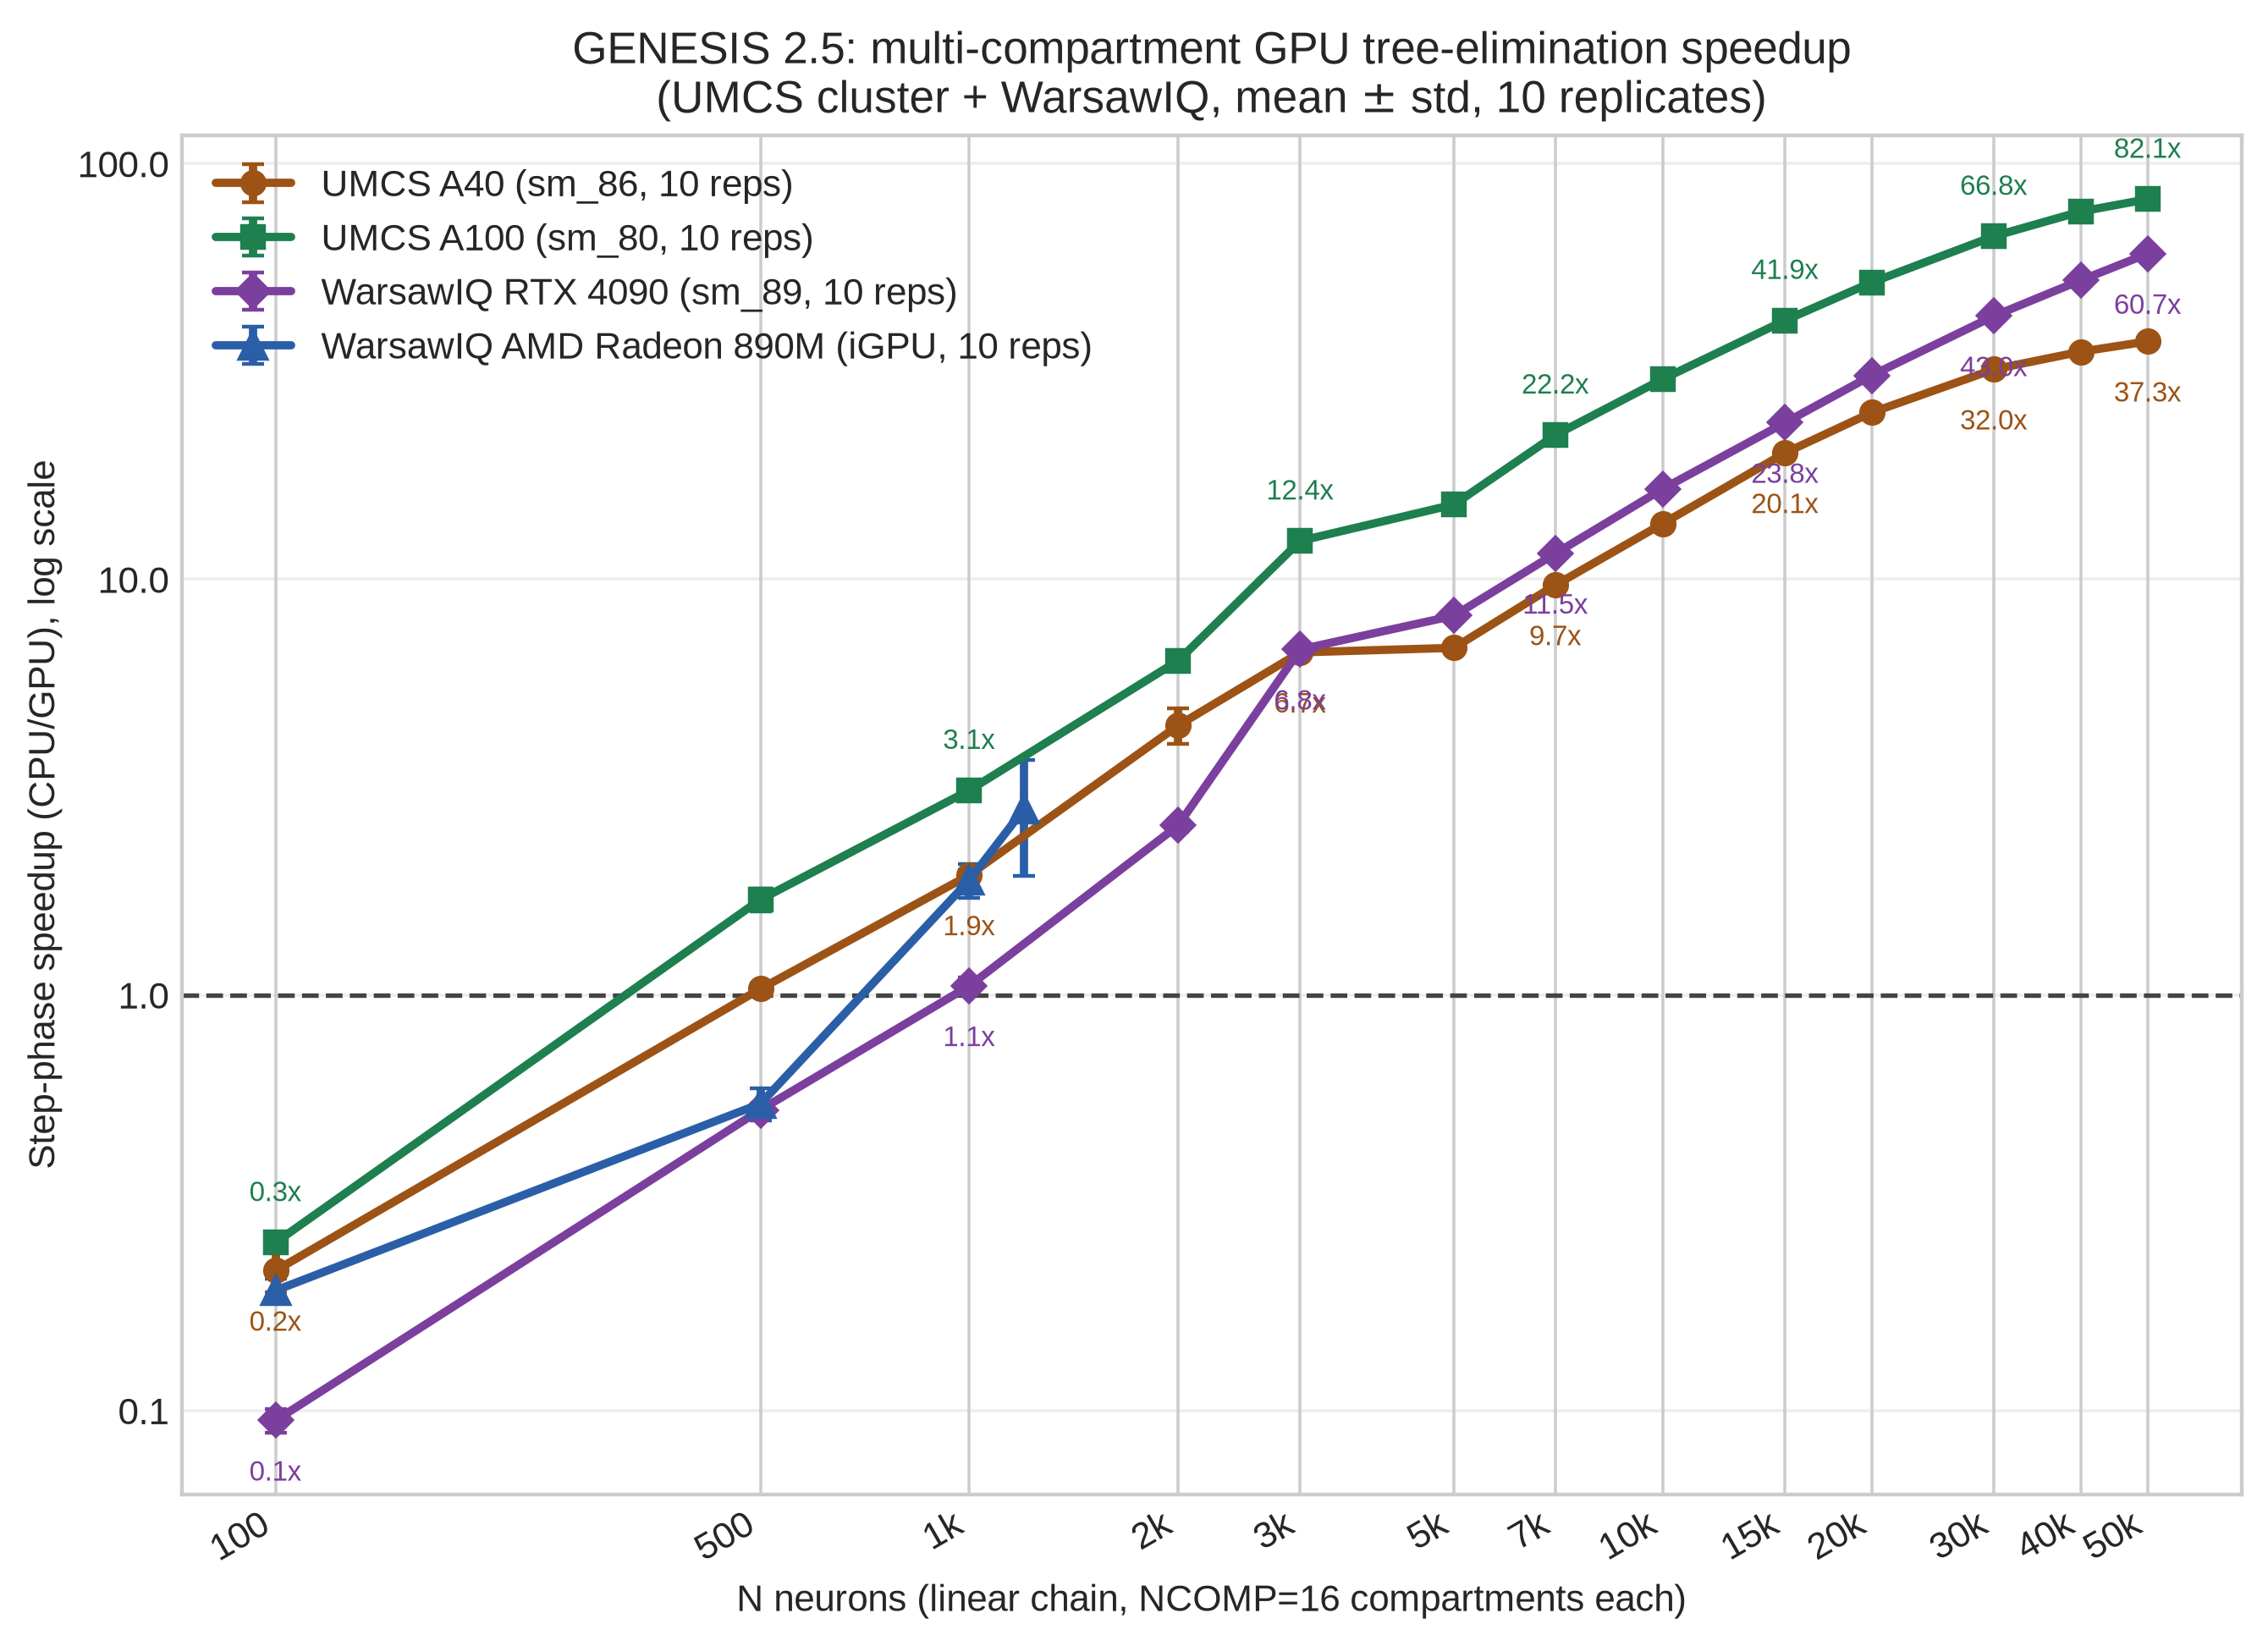
\includegraphics[width=0.98\textwidth]{fig10_multicompartment_speedup.png}
\caption{Multi-compartment GPU tree-elimination speedup vs.\ CPU (mean $\pm$ std, 10 replicates; log-log), UMCS A40/A100, sweeping $N$ at \texttt{NCOMP}\,$=16$ (linear-chain). Colour identifies the card, line style the metric: solid = step-phase (simulation loop only), dashed = end-to-end (whole process, including model construction). Both cards start below CPU parity and cross it near $N\approx500$--$1000$. The step-phase curves keep climbing to $80.8\times$ (A100) and $37.3\times$ (A40) without plateauing, but the end-to-end curves flatten near $3.9\times$ and $3.6\times$: at $K=200$ steps the unaccelerated construction phase bounds the achievable speedup, and only the step-phase curves measure the kernel itself. The two cards nearly coincide end-to-end despite the A100's large step-phase lead, as expected for an fp32 kernel using no tensor cores.}
\label{fig:multicomp_speedup}
\end{figure}

\textbf{Population-scale model construction was $O(n^2)$; now $O(n)$.} Pushing the multi-compartment benchmark toward the $\sim$31\,000-neuron Blue Brain Project scale~\cite{markram2015reconstruction} exposed a defect independent of GPU support: building $N=31\,000$ 17-compartment neurons (527\,000 compartments) did not finish within 900\,s, though Table~\ref{tab:multicomp} only required 160\,000. Profiling found a fitted exponent of $2.31$ ($O(n^2)$), traced to five pre-existing linear-scan-per-element patterns in core GENESIS code (element creation, path resolution, \texttt{hsolve} SETUP), none GPU-specific: each rescanned siblings, paths, or compartments in $O(n)$ where hashing or amortized growth would do. We fixed all five with hash-based lookups, load-factor rehashing, and geometric growth. Table~\ref{tab:construction_scaling} and Fig.~\ref{fig:construction_scaling} show a fitted exponent of $0.99$ after, effectively linear, extended to $N=100\,000$ (1.7~million compartments): the 527\,000-compartment population now builds in $14.6\pm0.2$\,s, down from not finishing, and the 1.7-million-compartment population in $51.5\pm0.6$\,s. Changes were verified to produce byte-identical output on every validation script, confirming a pure performance fix; full diagnosis in \path{genesis/src/hines/GPU_HINES_SOLVE_DESIGN.md}.

\begin{table}[!h]
\centering
\small
\begin{tabular}{|r|r|r|r|r|}
\hline
\textbf{$N$} & \textbf{total comps} & \textbf{before (s)} & \textbf{after: mean$\pm$std (s)} & \textbf{CV} \\
\hline
1\,000   & 17\,000    & 0.82    & 0.57 $\pm$ 0.08  & 13.2\% \\
\hline
2\,000   & 34\,000    & 2.03    & 0.93 $\pm$ 0.003 & 0.3\% \\
\hline
4\,000   & 68\,000    & 8.24    & 1.83 $\pm$ 0.04  & 1.9\% \\
\hline
8\,000   & 136\,000   & 105.45  & 4.08 $\pm$ 0.03  & 0.7\% \\
\hline
16\,000  & 272\,000   & did not finish (60\,s+)  & 7.54 $\pm$ 0.02  & 0.2\% \\
\hline
31\,000  & 527\,000   & did not finish (900\,s+) & 14.57 $\pm$ 0.18 & 1.2\% \\
\hline
50\,000  & 850\,000   & --                       & 23.80 $\pm$ 0.32 & 1.3\% \\
\hline
70\,000  & 1\,190\,000 & --                      & 34.25 $\pm$ 0.44 & 1.3\% \\
\hline
100\,000 & 1\,700\,000 & --                      & \textbf{51.48 $\pm$ 0.61} & 1.2\% \\
\hline
\end{tabular}
\caption{Model-construction wall time (construction + \texttt{hsolve} SETUP + one step), \protect\path{hh_branching_multicompartment_benchmark.g}, local machine, before vs.\ after the five fixes. ``After'': mean $\pm$ std, 3 replicates; ``before'': single replicate, not re-measured beyond $N=8000$ (``--'' = never attempted). Fitted exponent: $2.31$ before, $0.99$ after. Raw data: \protect\path{experiments/data/construction_scaling_before_after.csv}.}
\label{tab:construction_scaling}
\end{table}

\begin{figure}[!h]
\centering
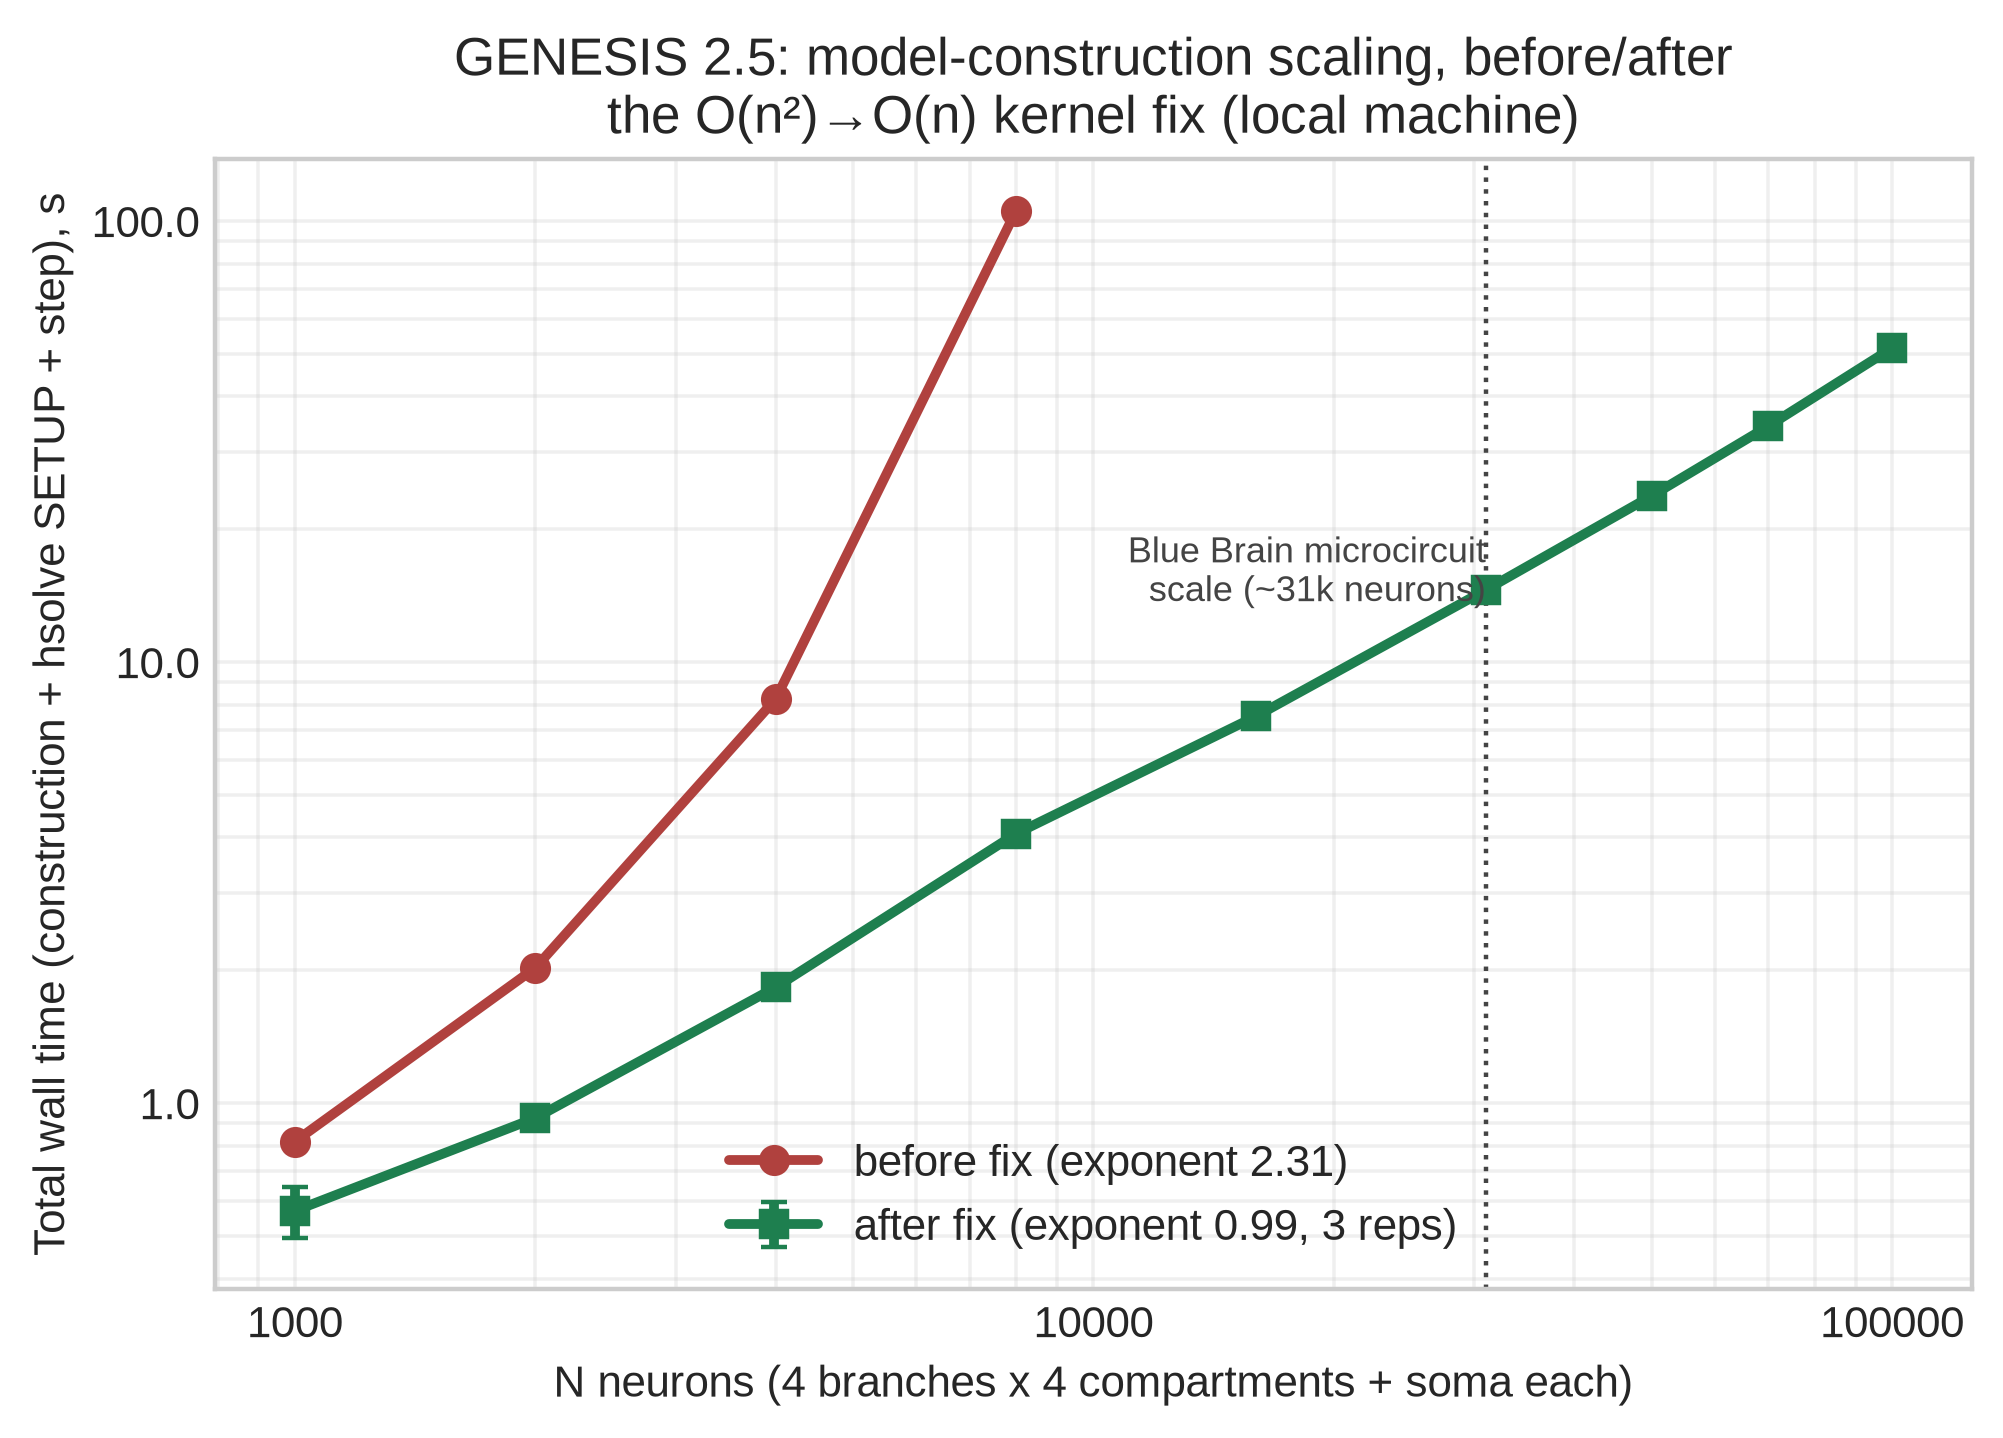
\includegraphics[width=0.8\textwidth]{fig11_construction_scaling.png}
\caption{Model-construction wall time vs.\ $N$, log-log, before (single replicate) and after (mean $\pm$ std, 3 replicates) the five $O(n^2)$ fixes, extended to $N=100\,000$. The ``before'' series stops at $N=8000$: larger $N$ did not finish within the tested budget.}
\label{fig:construction_scaling}
\end{figure}

\textbf{Speedup grows with simulation length.} Model construction is a fixed one-time cost, so end-to-end speedup depends on run length. Sweeping $K$ at fixed $N=5000$ (Fig.~\ref{fig:ksweep}) shows end-to-end speedup rising toward the step-phase ceiling: the accelerator pays off most for the long runs typical of real modeling studies (\path{experiments/data/campaign_ksweep.csv}).

\textbf{The multi-compartment figures are a floor set by the benchmark, not a ceiling set by the kernel.} The sweeps above use $K=200$ ($K=100$ for $N\geq5000$), which at $dt=50\,\mu$s is 5--10\,ms of simulated activity --- short enough that fixed costs dominate both arms. Repeating the measurement at $N=10\,000$ over a range of $K$ (Table~\ref{tab:mcksweep}) separates them: end-to-end speedup rises from $4.3\times$ at $K=200$ to $57.0\pm0.9\times$ at $K=5000$, and step-phase from $13.7\times$ to $116.2\times$. Both grow because the one-time costs they contain --- model construction for the end-to-end figure, buffer setup and the single batched dispatch for the step-phase figure --- are amortized over more steps.

Fitting fixed and marginal costs to the sweep separates them directly: construction is $\approx$1.3\,s on both arms, while the marginal cost of one step is $2.31\times10^{-2}$\,s on the CPU against $1.42\times10^{-4}$\,s on the GPU, a ratio of $163\times$. The device-side profile agrees independently, reporting $140.4\,\mu$s per step for the two tree kernels. The GPU arm reproduces the CPU voltages to $\sim$$10^{-7}$\,V at $K=5000$, the same fidelity as the short runs, so this is amortization rather than skipped work.

We report the short-$K$ figures in Table~\ref{tab:multicomp} because they are what the standing benchmark measures, but they understate what the kernel delivers in any realistic study: a 250\,ms simulation of this population already reaches $57\times$ end-to-end.

\begin{table}[!h]
\centering
\small
\begin{tabular}{|r|r|r|r|}
\hline
\textbf{$K$ steps} & \textbf{CPU (s)} & \textbf{GPU (s)} & \textbf{End-to-end} \\
\hline
200   & 5.86   & 1.37 & 4.28 $\pm$ 0.12 \\
\hline
500   & 13.00  & 1.42 & 9.18 $\pm$ 0.25 \\
\hline
1\,000  & 24.87  & 1.49 & 16.73 $\pm$ 0.36 \\
\hline
2\,000  & 48.03  & 1.63 & 29.48 $\pm$ 0.91 \\
\hline
5\,000  & 116.75 & 2.05 & \textbf{57.01 $\pm$ 0.88} \\
\hline
\end{tabular}
\caption{End-to-end wall clock against simulation length, $N=10\,000$ neurons $\times$ 16 compartments (160\,000 compartments), UMCS A40, mean $\pm$ std over 5 replicates, both arms timed identically. The fixed cost each arm carries --- $\approx$1.3\,s of model construction --- is unchanged across the sweep, so the speedup rises as $K$ grows: at $K=200$ construction is most of the GPU run, at $K=5000$ it is under a tenth of it. Raw data: \protect\path{cluster_bringup/logs/multicomp_ksweep_inf02_A40_20260816.csv}, produced by \protect\path{cluster_bringup/55_multicomp_ksweep.sh}.}
\label{tab:mcksweep}
\end{table}

\begin{figure}[!h]
\centering
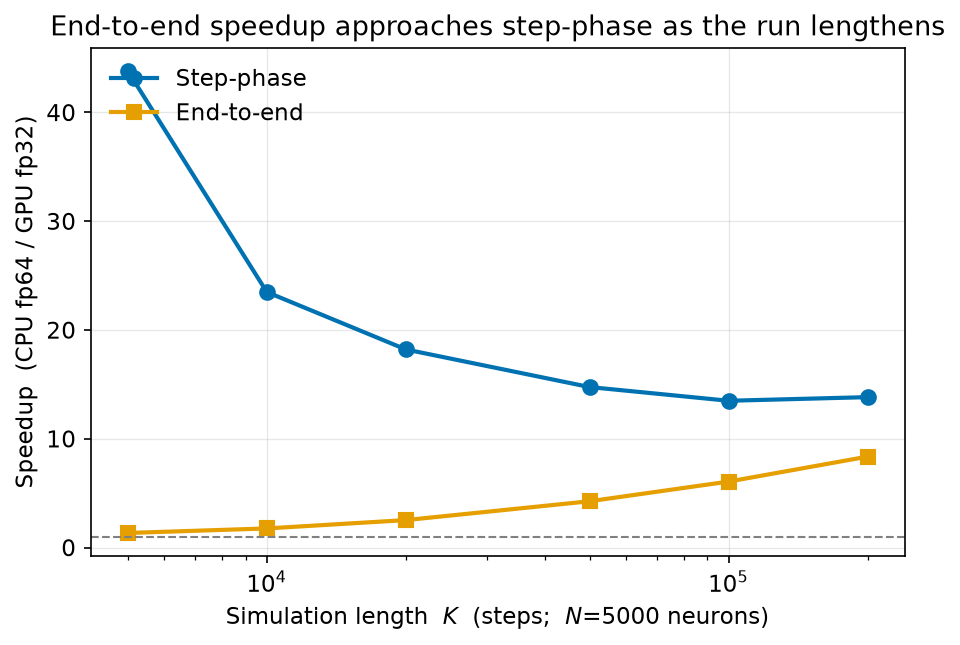
\includegraphics[width=0.8\textwidth]{fig_campaign_ksweep.png}
\caption{Speedup vs.\ simulation length $K$ at fixed $N=5000$. As the run lengthens, the one-time model-construction cost amortizes and the end-to-end speedup approaches the step-phase (simulation-only) speedup.}
\label{fig:ksweep}
\end{figure}

\textbf{Reproducing the PGENESIS scaling result.} The existing MPI path is unaffected; a strong-scaling sweep ($N=2400$ HH neurons, $P=1$--$24$ ranks, 12-core/24-thread host) gives near-ideal scaling at $P=2$ ($E_P=0.95$), an efficiency knee near $P\approx5$, and a recommended $P=4$--$8$ ($3.1$--$4.0\times$, 50--78\% efficiency) for this problem size.

\textbf{Head-to-head against NEURON and CoreNEURON.} The speedups above are internal (GPU vs.\ CPU within GENESIS) and say nothing about how GENESIS compares with other simulators. We therefore ran the Vogels--Abbott COBAHH network~\cite{vogels2005signal,brette2007simulation} in GENESIS (\path{Scripts/VAnet2}) and in the reference NEURON implementation (ModelDB~83319, \path{NEURON/cobahh}) on the same cluster node, all arms single-threaded on CPU (Table~\ref{tab:coreneuron}). GENESIS~2.5 completes the 5.0\,s simulation in $46.9\pm2.1$\,s, $1.63\pm0.07\times$ faster than CoreNEURON and $2.04\pm0.09\times$ faster than NEURON~9.0.2. CoreNEURON is in turn $1.25\times$ faster than NEURON~9.0.2, the expected ordering, which indicates the CoreNEURON arm is configured correctly rather than accidentally handicapped.

Because these are independent implementations of one benchmark, equivalence was established rather than assumed. Both networks have 4000 single-compartment cells (3200 excitatory, 800 inhibitory) and 80 synapses per cell; both are driven externally for the first 50\,ms only and then run on recurrent activity alone; both use $dt=0.05$\,ms for 5.0\,s. Critically, both settle into the same dynamical regime --- $26.8$\,Hz mean firing rate in GENESIS (536\,600 spikes) against $27.9$\,Hz in NEURON (558\,824), a 4\% difference --- so neither is doing materially less synaptic work than the other. Measuring the GENESIS rate required instrumenting every spikegen: the benchmark records membrane potential from three cells, two of which lie on the edge and corner of the grid where distance-dependent connectivity leaves them underconnected, and they fire at $7.6$ and $0.6$\,Hz against $15.8$\,Hz centrally.

The stock NEURON benchmark cannot run under CoreNEURON at all: its sodium and potassium channels are ChannelBuilder objects reconstructed inside the interpreter, and CoreNEURON, having no interpreter, aborts in \texttt{nrn\_setup} with \texttt{"nahh mechanism does not exist"}. We transcribed both channels into NMODL; the transcription is exact, reproducing the published COBAHH rate equations at $V_T=-63$\,mV, and CoreNEURON then yields a spike train byte-identical to NEURON's with the same compiled channels. Harness, mechanisms and full method are in \path{cluster_bringup/coreneuron/}.

This comparison establishes a single-core baseline only. CoreNEURON targets GPU and multi-rank MPI execution, and exercises neither here; the GENESIS arm is likewise its CPU arm, since VAnet2 cannot yet use the accelerator efficiently (Section~2.1).

\begin{table}[!h]
\centering
\small
\begin{tabular}{|l|l|r|r|}
\hline
\textbf{Simulator} & \textbf{Channels} & \textbf{Wall (s)} & \textbf{Spikes} \\
\hline
GENESIS 2.5 (VAnet2) & tabulated & \textbf{46.9 $\pm$ 2.1} & 536\,600 \\
\hline
CoreNEURON 9.0.2 & compiled NMODL & 76.5 $\pm$ 0.3 & 558\,824 \\
\hline
NEURON 9.0.2 & compiled NMODL & 95.8 $\pm$ 0.2 & 558\,824 \\
\hline
NEURON 9.0.2 & ChannelBuilder & 123.3 & 574\,138 \\
\hline
NEURON 8.0.2 & ChannelBuilder & 76.5 & -- \\
\hline
\end{tabular}
\caption{Vogels--Abbott COBAHH network, 4000 single-compartment cells, 80 synapses per cell, $dt=0.05$\,ms, 5.0\,s simulated, UMCS node inf03, all arms single-threaded CPU. Mean $\pm$ std over 3 replicates for the top three rows; the two ChannelBuilder rows are single runs, shown for reference only. GENESIS~2.5 is $1.63\pm0.07\times$ faster than CoreNEURON. The two simulators reach the same activity regime (26.8 vs.\ 27.9\,Hz), so the wall times reflect comparable work. All NEURON and CoreNEURON replicates returned an identical spike count, confirming the runs are deterministic. NEURON~8.0.2 is included because its pip distribution ships the CoreNEURON Python interface but not the engine, so the CoreNEURON arm requires NEURON~9. Harness: \protect\path{cluster_bringup/coreneuron/}.}
\label{tab:coreneuron}
\end{table}

Full replication steps and raw data are in \path{paper/docs/REPLICATION.md} and the self-contained \path{experiments/} package.

\item Impact

GENESIS/PGENESIS users with channel-kinetics-heavy models now have a path to GPU acceleration (Section~3) without migrating models, SLI scripts, or MPI workflows. That is the principal barrier an architecturally different successor such as MOOSE would otherwise impose. The three Hines-solver defects fixed along the way (Section~2) are independent of GPU support and affect any multi-neuron \texttt{hsolve} configuration: before the fix, \texttt{inject}-driven voltage transients were silently suppressed for every neuron but the first, with no error raised. That defect predates this release and is now fixed for any multi-neuron \texttt{hsolve} user, whether or not they use an accelerator.

Bringing up the accelerator backends surfaced four confounds: a GUI-linked binary, a benchmark that never dispatches to the kernel, CPU-timer semantics that overstate GPU-blocked wait as compute, and an off-by-one \texttt{argc} guard. Each produced a false reading at some point, and the wall-clock protocol built to catch them should generalize to any future GENESIS accelerator backend. On the UMCS cluster this scaled to 10-replicate statistical rigor for both kernels (Tables~\ref{tab:cuda}, \ref{tab:multicomp}), the multi-generation GPU comparison the cluster access was meant to provide. The dominant early cost was a broken $O(N)$ scheduler loop leaving neurons $2\ldots N$ unabsorbed and re-scheduled every step; fixing it is what makes Section~3's numbers possible. A further, structural limit remained: the multiloop kernel updates each compartment independently, so it only works for single-compartment networks. \texttt{hines\_tree\_eliminate} (Section~2.1, Section~3) closes that gap for population-scale simulation, parallelizing across neurons rather than within one tree.

The accelerator is deliberately scoped, and the scope is worth stating precisely rather than leaving to be discovered. Both kernels interpret the \texttt{hsolve} opcode program directly and implement the five opcodes a Hodgkin--Huxley \texttt{tabchannel} model driven by current injection produces. Compartments needing anything else --- synaptic channels, a \texttt{spike} element, GHK, calcium concentration pools --- are detected at \texttt{SETUP} and computed on the CPU, the accelerator declining that \texttt{hsolve} and reporting why. Validating this on a published network model exposed a fourth latent defect: the detection existed but its result was never consulted, so such compartments were dispatched to a kernel that mis-parses their opcode stream, giving wrong voltages from the first step with no error raised. It affected none of the benchmarks reported here, since none uses those elements; it affects any real network model that does. The check is now enforced, and the boundary it enforces is the honest statement of what this release accelerates.

Pushing toward the Blue Brain Project's scale~\cite{markram2015reconstruction} turned up a defect entirely separate from the GPU work: five pre-existing linear-scan patterns compounding into $O(n^2)$ model-construction time (Section~3). None is accelerator-specific, so fixing all five benefits any GENESIS/PGENESIS user building a large model: a second latent defect found only because this work pushed the codebase to a scale it had apparently never seen before.


\item Conclusions

GENESIS 2.5 adds opt-in OpenCL and CUDA acceleration to GENESIS 2.4/PGENESIS 2.4 for Hodgkin--Huxley \texttt{tabchannel} models, without changes to model files, SLI scripts, or MPI workflows (Section~3 reports speedup and fidelity for both integrated-GPU and cluster-class hardware). Beyond the single-compartment multiloop kernel, \texttt{hines\_tree\_eliminate} extends acceleration to axially-coupled multi-compartment trees at population scale; the single-detailed-cell regime is not helped by this design, which we measure and report rather than omit.

The release also carries four correctness fixes independent of accelerator use, benefiting any GENESIS/PGENESIS user. Three are latent Hines-solver defects that silently suppressed \texttt{inject}-driven voltage transients in any multi-neuron \texttt{hsolve}. The fourth is in the accelerator dispatch itself: compartments using opcodes the kernels do not implement were sent to the GPU anyway, producing silently wrong results; they are now detected and computed on the CPU. Separately, five pre-existing linear-scan patterns compounding into $O(n^2)$ model-construction time are fixed, restoring linear scaling and making population-scale models buildable at all.

Development continues along three lines: intra-tree parallelism (e.g.\ cyclic reduction) for the single-detailed-cell regime; extending kernel opcode coverage so synaptically coupled networks are accelerated rather than declined; and batching dispatch across \texttt{hsolve} elements, which the common one-solver-per-cell idiom currently defeats. Packaging into a container-based on-premise/cloud deployment pipeline~\cite{chlasta2023pipeline} is in progress.

\end{enumerate}

\section*{Acknowledgements}
\label{}

The authors thank the Maria Curie-Sk\l{}odowska University (UMCS) in Lublin and
the LubMAN UMCS computing centre for access to the ``Lunar'' cluster (NVIDIA A100
and A40 GPU nodes) at the UMCS Institute of Mathematics, commissioned in
2015~\cite{umcs_lunar2015} and since upgraded with the GPU nodes used in this
work, and Karol S.~Karpowicz and Prof.~Przemys\l{}aw Stpiczy\'nski
for provisioning and support of the compute environment on which the CUDA backend
was built and validated. The authors also thank WarsawIQ for the AMD Radeon~890M
integrated GPU used for the laptop-class benchmarks reported here.

%% The Appendices part is started with the command \appendix;
%% appendix sections are then done as normal sections
%% \appendix

%% \section{}
%% \label{}

%% References:
%% If you have bibdatabase file and want bibtex to generate the
%% bibitems, please use
%%
%%  \bibliographystyle{elsarticle-num} 
%%  \bibliography{<your bibdatabase>}

%% else use the following coding to input the bibitems directly in the
%% TeX file.

\begin{thebibliography}{9}

\bibitem{bower1998}
Bower~JM, Beeman~D.
\textit{The Book of GENESIS: Exploring Realistic Neural Models with the GEneral NEural SImulation System}.
Springer, 1998.

\bibitem{g3_dev_plans}
GENESIS 3 Development Plans.
\url{http://www.genesis-sim.org/GENESIS/G3/G3-dev-plans.html}

\bibitem{cornelis2011}
Cornelis~H, Coop~AD, Rodriguez~AL, Beeman~D, Bower~JM.
GENESIS 3.0 functionality enhanced by interface to multiple types of database.
\textit{BMC Neuroscience} 2011, 12(Suppl 1):P15.

\bibitem{cornelis2008cbi}
Cornelis~H, Edwards~M, Coop~AD, Bower~JM.
The CBI architecture for computational simulation of realistic neurons and circuits in the GENESIS 3 software federation.
\textit{BMC Neuroscience} 2008, 9(Suppl 1):P88.

\bibitem{cornelis2007dendrite}
Cornelis~H, Lu~H, Esquivel~A, Bower~JM.
Modeling a single dendritic compartment using Neurospaces and GENESIS-3.
\textit{BMC Neuroscience} 2007, 8(Suppl 2):P3.

\bibitem{cornelis2013interop}
Cornelis~H, Bampasakis~D, Steuber~V, Bower~JM.
Interoperability in the GENESIS 3.0 Software Federation: the NEURON Simulator as an Example.
\textit{BMC Neuroscience} 2013, 14(Suppl 1):P33.

\bibitem{arbor2019}
Akar~NA, Cumming~B, Karakasis~V, K\"usters~A, Klijn~W, Peyser~A, Yates~S.
Arbor -- A Morphologically-Detailed Neural Network Simulation Library for Contemporary High-Performance Computing Architectures.
In: \textit{27th Euromicro International Conference on Parallel, Distributed and Network-Based Processing (PDP)}, 2019, pp.~274--282. doi:10.1109/EMPDP.2019.8671560.

\bibitem{kumbhar2019coreneuron}
Kumbhar~P, Hines~M, Fouriaux~J, Ovcharenko~A, King~J, Delalondre~F, Sch\"urmann~F.
CoreNEURON: An Optimized Compute Engine for the NEURON Simulator.
\textit{Frontiers in Neuroinformatics} 2019, 13:63. doi:10.3389/fninf.2019.00063.

\bibitem{markram2015reconstruction}
Markram~H, Muller~E, Ramaswamy~S, et al.
Reconstruction and Simulation of Neocortical Microcircuitry.
\textit{Cell} 2015, 163(2):456--492. doi:10.1016/j.cell.2015.09.029.

\bibitem{vogels2005signal}
Vogels~TP, Abbott~LF.
Signal Propagation and Logic Gating in Networks of Integrate-and-Fire Neurons.
\textit{Journal of Neuroscience} 2005, 25(46):10786--10795. doi:10.1523/JNEUROSCI.3508-05.2005.

\bibitem{brette2007simulation}
Brette~R, Rudolph~M, Carnevale~T, Hines~M, Beeman~D, Bower~JM, et al.
Simulation of networks of spiking neurons: A review of tools and strategies.
\textit{Journal of Computational Neuroscience} 2007, 23(3):349--398. doi:10.1007/s10827-007-0038-6.

\bibitem{chlasta2023pipeline}
Chlasta~K, Sochaczewski~P, W\'ojcik~GM, Krejtz~I.
Neural simulation pipeline: Enabling container-based simulations on-premise and in public clouds.
\textit{Frontiers in Neuroinformatics} 2023, 17:1122470. doi:10.3389/fninf.2023.1122470.

\bibitem{umcs_lunar2015}
Maria Curie-Sk{\l}odowska University (UMCS), Instytut Matematyki.
Superkomputer LUNAR uruchomiony w Instytucie Matematyki UMCS.
\url{https://www.umcs.pl/pl/aktualnosci,57,superkomputer-lunar-uruchomiony-w-instytucie-matematyki-umcs,27879.chtm}, 2015.

\end{thebibliography}


\section*{Current executable software version}
\label{}

Not applicable; this release is distributed as source code only (see Current code version above).


\end{document}
\endinput
%%
%% End of file `SoftwareX_article_template.tex'.
